From the analysis of quality requirements it was revealed that Reliability(QR), Maintainability(QR) and Flexibility(QR) were all deemed to be of high or medium priority. These factors are influenced by the software having low-coupling and robust systems. Investing time on technical design and architecture at the start of the project allows for reduced cost of refactoring in the long term; This will be mentioned more under Design Post-Mortem. For this reason it was deemed an important focus on architecture throughout the project.

\subsection{Data Model}
Featured below is the UML Class diagrams of model objects to be implemented in Java. They were made from analysis of Data Modelling and modified to meet the needs of Functional Requirements. This model does not represent the full system but just the core classes in the model. All attributes can be assumed to have getters or setters unless stated otherwise and the functions mention are examples of additional functionality and may not be reflective of the final system completely.
Each of these core classes inherits from UUID Entity that gives the object a unique identifier that is used internally within the system that is discussed further in Section \ref{subsec:Architecture}.

\subsubsection{Menu}

\begin{wrapfigure}{l}{0.3\textwidth}
	\centering
	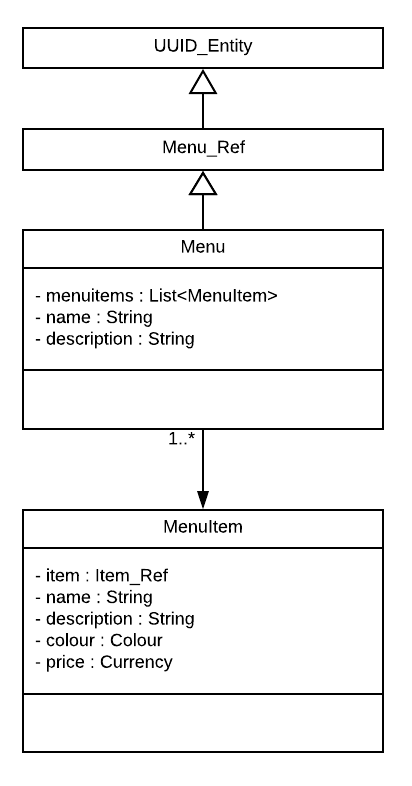
\includegraphics[width=0.25\textwidth]{images/data_model/menu.png}
	\caption{This is a figure caption.} \label{fig:UML_Menu}
\end{wrapfigure}


\lipsum[2-3]

\subsubsection{Item}
\subsubsection{ItemTag}
\subsubsection{StockInstance}
\subsubsection{Order}

\subsection{Architecture} \label{subsec:Architecture}
\subsection{Design Post-Mortem}